\onecolumn
\chapter*{Il Libro}
\begin{racconto}
  ``La stanza era fredda e fiocamente illuminata da tre candele su un
  candelabro di bronzo. La fiamma nel camino si era assopita da tempo
  lasciando alla brace il ruolo di protagonista. Don Michele era
  cos\`{\i} intento a copiare il vecchio testo che non si rese conto
  del suo respiro che si condensava davanti alle pergamene.
  
  La stanza era invasa da ombre che gettavano in ogni angolo un cesto
  di paure. Michele ripeteva sottovoce ci\`o che la sua mano e la
  sua penna andavano vergando sul foglio. Egli non si sarebbe mai
  aspettato di cadere nel baratro della dannazione. Era un servo
  fedele di Ryless, del suo Pontefice e del suo Vescovo, e come suo
  braccio destro credeva d'essere un protetto dal Messia.
  
  Le ombre si condensarono dietro di lui e un vento gelido mosse le
  fiamme delle candele e ravviv\`o i ceppi moribondi del camino. Don
  Michele non si ridest\`o dal suo lavoro mentre i passi silenziosi
  prendevano forma dietro di lui. Una mano gelida si pos\`o sulla
  sua spalla sinistra. Don Michele si volt\`o e il suo urlo, un urlo
  che non emise suono, gli mor\`{\i} in gola. I suoi occhi
  strabuzzarono mentre osservava la figura davanti a lui.
  
  --Chi... Chi Sei?-- mormor\`o
  
  --Ciao, giovane Michele, ti ho spaventato?-- disse la figura, una
  donna bellissima dai capelli rossi avvolta da un sottile velo nero
  che non lasciava niente da immaginare.
  
  --Chi sei, e cosa fai nelle mie stanze, donna?-- rispose con il cuore
  che martellava come un tamburo.
  
  --Donna? Non sono donna pi\`u di quanto non lo sia tu, Michele--
  
  --Che cosa vuoi dire?--
  
  --Troppe domande e tutte inutili, Michele. Piuttosto chiediti cosa
  voglio da te e cosa posso fare per te-- continu\`o la donna
  
  --Cosa vuoi da me?-- chiese allora Michele, stringendo, cos\`{\i} forte
  da farsi sanguinare le mani, il pugnale: il simbolo della morte di
  Ryless.
  
  --Voglio che abbandoni Ryless. Voglio la Chiesa, tutta, ai miei
  ordini.  E voglio che tu sia mio--
  
  --No! Mai! La mia fede \`e grande, pi\`u grande di qualunque
  potere o demone. Esci di qui!--
  
  --Fede??-- La donna inizi\`o a ridere sguaiatamente, ma nessun
  suono usciva dalla stanza.
  
  --Ryless avrebbe desiderato, e lo desidera ancora, un potere come il
  mio.  \`E un debole, non sa neppure ci\`o che accade nei suoi amati
  cieli, non sa neppure cosa tramano i suoi adorati Gabriel e Lucifer,
  \`e un inetto che passa il suo tempo con Antiochio, sorseggiando 
  Phyluf--Herhu tra una partita a carte e una a morra.--
  
  --Menzogne, lui \`e nostro padre e nostra madre; lui \`e la
  nostra guida, la salvezza che ci illumina con la sua grazia!-- si
  difese con forza, Don Michele; ma gi\`a vacillava sull'orlo della
  disperazione.
  
  --Gi\`a, menzogne! Michele, Ryless non ha creato nulla che io non
  possa creare mille volte pi\`u bello e potente. Ti dimenticherai
  di lui, credimi, e noi ci ameremo presto. Mentre attendi, mio
  piccolo amore, scendi nella cripta e apri il sarcofago di San
  Fulgenzio e togli l'elmo dalla sua testa, poi tutto ti si aprir\`a
  davanti. Dopo potrai scegliere il tuo destino--
  
  La donna si accost\`o a don Michele, ormai paralizzato, e lo
  baci\`o sulle labbra.
  
  Le labbra di lei erano di fuoco, roventi come la lava e taglienti
  come rasoi, e risvegliavano i sensi di Michele senza che egli
  potesse opporsi...
  
  Michele si accasci\`o di colpo, come morto. Dorm\`{\i}, sognando
  demoni e partite di carte e la donna dai capelli rossi che nei suoi
  incubi si trasformava in un terribile mostro dai denti aguzzi e
  dalle grandi ali di pipistrello, rosso come il sole al tramonto.
  
  Si ridest\`o ben prima delle odi del mattino, madido di sudore ed
  infreddolito.  Si ritrov\`o a pensare che tutto fosse stato un
  sogno, ma voltandosi nel letto trov\`o sul guanciale una ciocca di
  capelli rossi. Si alz\`o e indoss\`o la tunica e i calzoni, poi
  si avvi\`o verso le cantine. Ud\`{\i} la porta cigolare sinistramente
  ma non ci fece caso. Prese una lanterna dallo scaffale, la
  caric\`o ed accese lo stoppino. Scese silenziosamente sino alla
  cripta. L'umidit\`a era come un peso sulle spalle e rendeva
  difficile la respirazione.
  
  La luce della lanterna era fioca e non dissolveva le tenebre della
  tomba, ma Michele riusc\`{\i} lo stesso a raggiungere il sarcofago
  di granito. Pos\`o la lanterna a terra e spinse con forza. I suoi
  piedi scivolavano sulla muffa del pavimento e le sue unghie si
  spezzavano sul granito mentre il suo sangue cadeva in gocce grosse
  come perle.
  
  Finalmente vide il volto scheletrico di San Fulgenzio, adorno del
  suo elmo.  Il tanfo della morte lo invest\`{\i} come un cavallo in
  carica. Pose le sue mani sull'elmo e lo tir\`o con forza. L'elmo
  si stacc\`o insieme al cranio.
  
  --Ryless, cosa ho fatto!?-- bisbigli\`o, lasciando cadere il teschio
  e portandosi le mani, asciutte e disperate, alla testa.
  
  --Nulla di importante, ma lo hai fatto per me.-- La donna era
  comparsa alle sue spalle, la luce della lanterna non riusciva ad
  illuminarne il volto incorniciato dal rosso crine.
  
  --Mi hai ingannato!-- Inve\`{\i} Michele puntando il dito.
  
  --Su, Su! Non essere permaloso! Avrai ci\`o per cui sei venuto.--
  La donna sorrise mostrando i denti aguzzi. --Ti presento uno dei miei
  servi-- indic\`o l'oscurit\`a --Si chiama Arioch.--
  
  L'ombra vomit\`o un essere alto come un orco, con la pelle rossa e
  striata, le ali di pipistrello e il capo coronato da due corna
  massicce.
  
  --Ciao, Uomo!-- ghign\`o Arioch, mostrando una fila di robustissime
  zanne, bianche come ossa spolpate. Una colonna di fiamme si
  sprigion\`o dalle sue mani. Michele riusc\`{\i} appena in tempo ad
  attivare l'incantesimo di protezione, toccando il suo orecchino
  magico. Fu avvolto dalle fiamme, che lo abbracciarono in mille e
  pi\`u vortici, ma soltanto qualche lembo della sua tunica
  risent\`{\i} degli effetti della fiammata, restando bruciacchiato.
  
  --Dannato demone!-- imprec\`o con rabbia e paura.
  
  --Guarda dietro di te, Uomo!-- grugn\`{\i} il mostro, --Non farmi
  pentire di averti risparmiato--
  
  Michele si volt\`o e vide che si era aperta una crepa nel muro.
  Una luce biancastra filtrava, accompagnata da una sorta di ronzio.
  Michele l'attravers\`o abbacinato.
  
  Mentre i suoi passi rimbombavano nel corridoio, con le mani sfiorava
  le pareti, lisce e fredde, di un metallo mai visto. Di tanto in
  tanto trovava delle strane iscrizioni, dei dipinti con strane forme
  e porte di metallo che non pot\`e aprire in nessun modo.
  
  Cammin\`o per un tempo che gli sembr\`o infinito, finch\'e
  trov\`o il cammino sbarrato da una gigantesca parete di metallo.
  Prov\`o a spingere con tutte le sue forze fino a sentire i muscoli
  di braccia e gambe intorpidirsi.
  
  Poi url\`o. --Ecco! \`E tutto qui ci\`o che doveva distruggere la
  mia fede?-- chiese all'aria che respirava.
  
  --Chiedi aiuto, giovane Michele.-- risuon\`o nella sua mente
  cos\`{\i} forte da costringerlo a tapparsi le orecchie.
  
  --Aiuto, allora. Aiuto!-- ringhi\`o. Una rabbia poderosa, imponente,
  che mai avrebbe sospettato di poter manifestare, si impossess\`o di
  lui.
  
  --Spostati, ammasso di carne urlante.-- brontol\`o con sufficienza,
  spuntando dal nulla, Arioch.
  
  Il mostro colp\`{\i} l'uomo sul petto senza ferirlo, eruttando di nuovo
  le sue fiamme ma ora con tutto il suo potere. Il volto del mostro
  illuminato dal fuoco infernale era una maschera di piacere, dolore e
  follia.
  
  Michele avvert\`{\i} nel petto un caldo opprimente e cap\`{\i} di
  essere stato risparmiato. La parete dietro di lui si sciolse come
  lardo sulla brace.
  
  Un vortice di fumo comparve ed avvolse il Demone, che url\`o con
  odio.
  
  Il fumo si dissip\`o e Michele vide che il Demone era scomparso, e
  che al suo posto c'era ora un oggetto. Un pastorale.
  
  Lo raccolse e lo guard\`o impaurito. l'asta vibrava fra le sue
  mani come percorsa da una strana energia, ed era calda, viva. Lo
  rigir\`o fra le mani e si avvide della somiglianza del suo
  pastorale con quello del Vescovo.
  
  Una luce accecante lo invest\`{\i} e lo distolse dalle sue
  impressioni sul pastorale. Come ipnotizzato si diresse verso la
  fenditura che il demone aveva aperto nella parete. Michele aveva il
  braccio destro davanti a se, disteso, quasi a voler tastare la luce,
  sentirla. Con l'altra mano stringeva il pastorale che continuava a
  muoversi e contrarsi e respirare. La luce era fredda e quasi
  tagliente all'interno di quella enorme stanza.
  
  Davanti agli occhi gli si stagliava un gigantesco, monumentale cilindro
  di metallo che lo guardava con un enorme occhio rosso.
  
  --Quanto tempo \`e passato!-- risuon\`o una voce metallica,
  --Finalmente qualcuno con cui parlare--
  
  --Chi... Cosa?-- balbett\`o Michele
  
  --Io sono la memoria impotente di questo mondo. Io ho visto e
  registrato vita e morte e ricostruzione, e poi ancora vita. Io sono
  il cuore che batte.  Io sono...--
  
  La voce fece una pausa.
  
  --Solo.-- Continu\`o la voce --Da troppo tempo ormai.--
  
  --Ma...-- Michele aveva molte domande, e tutte gli morirono in gola.
  Cosa era quell'essere? Era vivo? Cosa voleva? Da quanto esisteva?
  
  --Io so che sono tante le tue domande, e che il tuo cuore batte
  troppo forte. Ma io non mi ricordo il calore di un essere vivente...
  Avvicinati, e se lo vorrai, ti sveler\`o la Verit\`a.--
  
  Michele si avvicin\`o passo dopo passo, lentamente, mentre il suo
  cuore sembrava non distinguere pi\`u un battito dall'altro. Il
  dimenarsi leggero e caldo del pastorale lo rassicurava. Sentiva il
  fuoco fluire dentro di s\`e.
  
  --Mostramela!-- grid\`o Michele, allargando le braccia. Dalla base
  dell'occhio saettarono migliaia di tentacoli che lo avvolsero come
  una gabbia di rovi e lo percorsero, lo sentirono, e gli mostrarono
  la Verit\`a. La verit\`a disperse il suo cuore. Per Sempre.
  
  Il pastorale cadde dalla sua mano, mentre viveva ci\`o che era
  stato.  Le macchine volanti. La nascita delle razze. L'arrivo di una
  nave dal cielo.  La rabbia della Terra.
  
  Vide colonne di fiamme alte decine di chilometri e nubi nere come
  l'oblio.  Sent\`{\i} il dolore, la paura, le lacrime e l'abbandono
  di un mondo. Url\`o fino a dimenticare quanto. Riemerse dal dolore
  nel suo letto, si sedette e dopo aver dissolto il torpore iniziale
  studi\`o il pastorale fra le mani. Era vivo, non c'era dubbio.
  
  --Arioch!-- chiam\`o. Un vortice di fumo scatur\`{\i} dall'asta, si
  condens\`o e l'Arioch apparve. --Chiama i tuoi demoni. Che scrivano
  ci\`o che mi \`e stato svelato.-- ordin\`o Michele.
  
  Arioch rispose sprezzante: --O forse potrei strapparti la carne a
  poco a poco--
  
  --Chiamali. Te lo ordino.-- ribad\`{\i}.
  
  I loro sguardi si incrociarono. I rossi occhi di Arioch sprizzavano
  fiamme di odio e dolore, che sfidavano la pazzia pura e semplice
  degli occhi azzurri di Michele. Dopo una eterna frazione di secondo
  Arioch chin\`o il capo, si inginocchi\`o e ringhi\`o di
  rabbia:
  
  --Agli ordini, Padrone!--
  
  L'istante successivo apparve un essere orribile, una sorta di
  ammasso cartilagineo dotato di otto arti peduncolati e di uno strano
  tentacolo. Il tentacolo si avvilupp\`o intorno alla testa di
  Michele ed inizi\`o a pulsare. Il Demone inizi\`o a gonfiarsi
  delle memorie del giovane, fino a occupare tutta la stanza. Una
  grossa pustola, ricolma di conoscenza.
  
  Il mostro aracnoide inizi\`o a scrivere, veloce come il vento, e
  mentre scriveva il sapere sui fogli, il suo ventre si sgonfiava.
  
  --Andiamo, ora, andiamo a trovare un defunto-- ghign\`o Michele
  rivolgendosi all'Arioch.
  
  --S\`\i, mio Signore-- rispose l'Arioch, quasi soddisfatto.
  
  Michele si diresse senza alcuna circospezione verso la stanza del
  suo superiore, si accost\`o alla porta salutando la guardia che la
  presidiava.  Il Vescovo di Rylex dormiva ancora.
  
  Michele lo dest\`o dolcemente: --Mia Eccellenza-- salut\`o con un
  inchino.
  
  --Oh, Michele. Perch\'e mi svegli cos\`{\i} presto?-- domand\`o
  assonnato l'anziano Vescovo.
  
  --Un funerale, Eccellenza.-- Michele sfoder\`o un sorriso
  sarcastico.  Il pastorale gli pulsava ancora tra le mani.
  
  --A quest'ora?-- domand\`o sbigottito il vecchio, --E di chi?--
  
  --Il suo, Eccellenza-- Il vecchio non fece in tempo a stupirsi che le
  mani di Michele si levarono. Il corpo del vescovo cominci\`o a
  contrarsi in preda alle convulsioni. Il torace gli si gonfi\`o,
  fino a lacerare la veste, la pelle, la gabbia toracica fino alla
  gola, soffocando i suoi lamenti. Il corpo del vecchio esplose,
  rivoltandosi come un guanto. Di quello che era stato l'arcivescovo
  di Rylex era rimasto un ammasso di visceri e ossa sanguinolente.
  
  Michele richiam\`o il suo Arioch e gli ordin\`o di uccidere la
  guardia all'ingresso. La porta si apr\`{\i} e, mentre Michele usciva,
  la testa della guardia implodeva con uno schiocco sordo sotto la
  stretta dell'Arioch.
  
  --Ora sparisci-- ordin\`o al demone. Michele torn\`o nelle sue
  stanze.  Dove prima c'era il demone gonfio di conoscenza si trovava
  il Libro. Sollev\`o il tomo fra le mani e pronunci\`o un
  vincolo, e poi un altro, e poi un altro ancora, e poi ancora, fino
  quasi a crollare esausto.
  
  --Ecco il Radix Malorum, la Radice di tutti i Mali. Lo custodir\`o
  e nessuno sapr\`a mai la Verit\`a.-- esclam\`o. Tra le nebbie
  della stanchezza che lo sommergevano vide apparire la donna dai
  capelli rossi. Nuda, bella, provocante.
  
  --E tu sarai mio-- disse sorridendo la donna.
  
  --S\`i, mio Signore-- rispose Michele perdendosi nel suo caldo
  abbraccio.''
\begin{figure*}[t]
\begin{center}
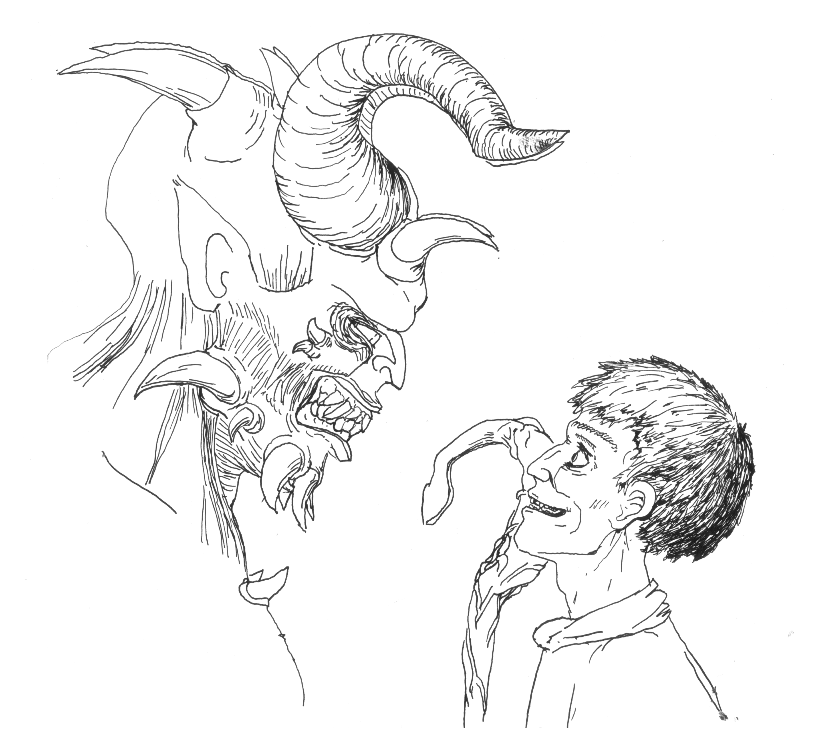
\includegraphics{michele_arioch.eps}
\end{center}
\end{figure*}

\end{racconto}

\twocolumn

%%% Local Variables: 
%%% mode: latex
%%% TeX-master: "manual"
%%% End: